\begin{figure}[t]
	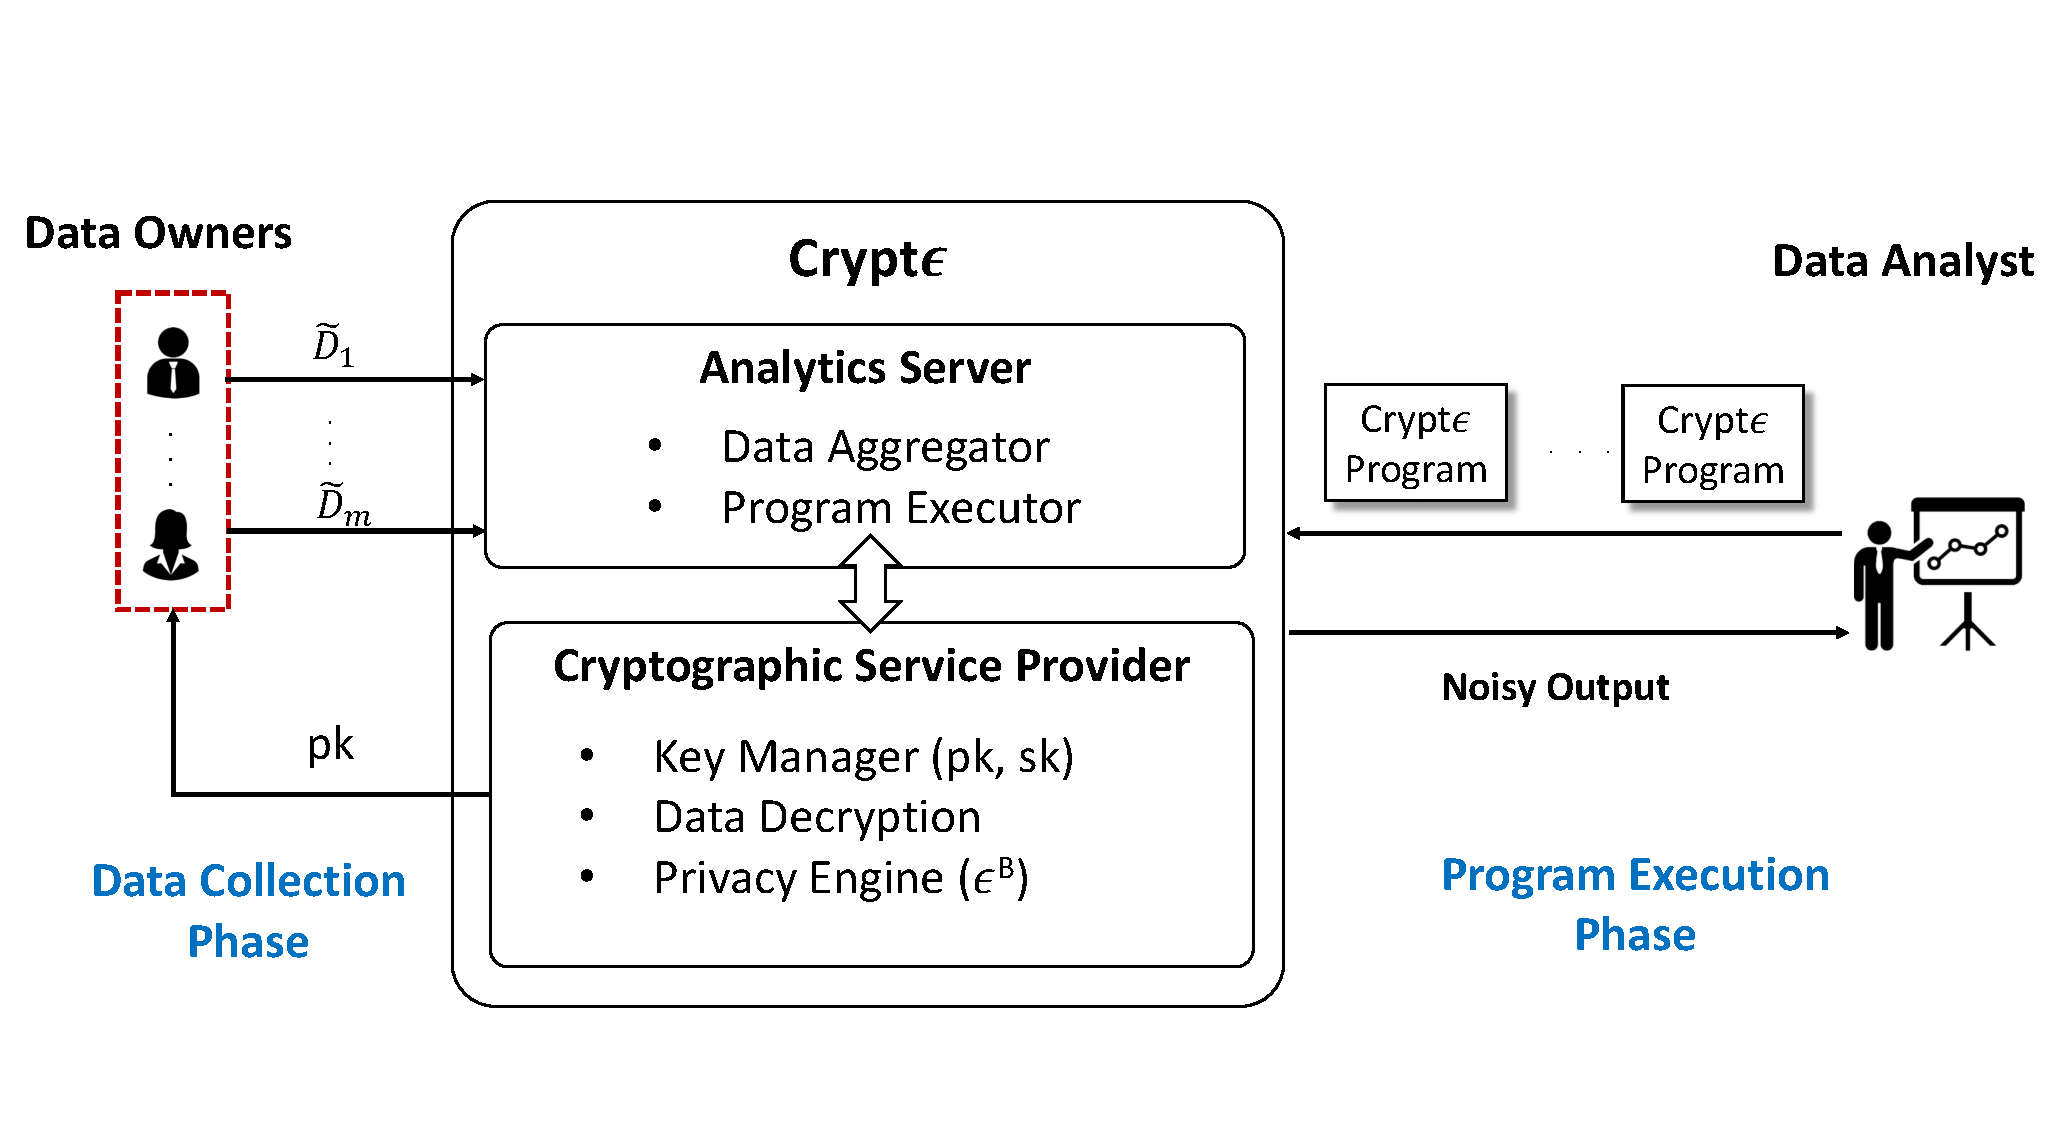
\includegraphics[width=0.9\columnwidth]{diag.pdf}\vspace{-5mm}
	\caption{\label{fig:system} Crypt$\epsilon$ System}% Setting: The  \textsf{AS} runs the Crypt$\epsilon$ programs. The \textsf{CSP} manages the cryptographic primitves. }
\end{figure}


\section{\system Overview}\label{sec:overview}
In this section, we describe the architecture of \system (Section~\ref{sec:arch}), the different modules in the system (Section~\ref{sec:modules}), and the trust assumptions made by our system (Section~\ref{sec:trust}). We end with a brief discussion justifying the design of \system (Section~\ref{sec:discuss-arch}). The key notations used in this paper are summarized in Table~\ref{Notations}.

\subsection{System Architecture}\label{sec:arch}
The architecture of \system is illustrated in Figure~\ref{fig:system}. A set of \textit{data owners} ${\textsf{DO}_i, i\in [m]}$ have private data records ${D_i, i \in [m]}$. \system permits data analysts to author and execute programs $P$ that satisfy differential privacy under the \cdp model without storing or computing on the private data records in the clear. \system achieves this by aggregating encrypted private records at the \textit{Analytics Server} (\textsf{AS}). Keys needed for encrypting private records and decrypting answers are managed by the \textit{Cryptographic Servide Provider} (\textsf{CSP}) so that the data owner need not participate in the differentially private computation.

\system operates in three phases: 
 \squishlist
 \item \textbf{Setup Phase}: In the first phase, data owners initializes the \textsf{CSP} with a privacy budget $\epsilon^B$, which is stored in the \textsf{CSP}'s \textit{Privacy Engine} module. Next, the  \textsf{CSP}'s \textit{Key Manager} module generates the key pairs for labHE $(sk,pk)$, publishes $pk$ and stores $sk$. 
 \item \textbf{Data Collection Phase}: In the next phase, each data owner encodes and encrypts their records using the \textit{Data Encoder} and \textit{Data Encryption} modules and sends the encrypted data records to the \textsf{AS}. The data owners are relieved of all other duties and can go completely off-line. The \textit{aggregator} module of the \textsf{AS} then aggregates these encrypted records into a single encrypted database $\boldsymbol{\tilde{\mathcal{D}}}$.
 \item \textbf{Program Execution Phase}: In this phase, the \textsf{AS} executes a \system program provided by the data analyst. \system programs (which are described in more detail in Sections~\ref{sec:primitives} and \ref{sec:implementation}) access the sensitive data using a restricted set of data transformations, that filter, count or group the sensitive data, and measurement primitives, which are differentially private operations to release noisy answers. A majority of the data transformation operations are executed wholly at the \textsf{AS}. However, every measurement operator requires an interaction with the \textsf{CSP} as it requires (a) decryption of the answer, and (b) a check that the the privacy budget is not exceeded. These two functionalities are achieved by the \textit{Decryption} and \textit{Privacy Engine} modules of the \textsf{CSP}.
 \squishend
 The \emph{Setup} and \emph{Data Collection} phases occur just once at the very beginning, every subsequent program  is handled via the corresponding  \emph{Program Execution} phase. We next detail the roles of the different modules in the data owners, the Analytics Server and the Cryptographic Service Provider.  


\begin{table}[t]
\centering
\caption {Notations}
\scalebox{0.8}{
 \begin{tabular}{l|l}  \toprule
 \multicolumn{1}{c}{\textbf{Symbol} } &  \multicolumn{1}{c}{\textbf{Explanations}}\\\midrule
\textbf{Boldface}& \text{- represents encrypted data}\\
$\tilde{}$ & \text{- represents one-hot-coding}  \\  $\hat{}$ & - represents a differentially private output  \\ $A$ &- an attribute  \\ $s_A$ &- size of domain of attribute $A$
\\$dom(A)=\{v_1,\ldots,v_{s_A}\}$ & - domain of attribute $A$\\ $ct_{A,i}$  &- \# \text{records with value $v_i$ for attribute} A\\ $m$   &- \text{\# number of data onwers}\\ $\boldsymbol{\tilde{\mathcal{D}}}$  &- \text{encrypted database with records in}\\&\text{  per-attribute one-hot-coding } \\ %$\mathcal{A}=\{\mathcal{A}_1,...\mathcal{A}_l\}$   &- \text{set of attributes in the schema of $\boldsymbol{\tilde{\mathcal{D}}}$}\\
$x \times y \text{ table } \mathbf{T}$   &- \text{an encrypted table  with $x$ records in}\\&\text{ one-hot-coding and $y$ columns one for}\\&\text{ each attribute; serves as one of the }\\&\text{ inputs to a transformation primitive}\\ $\mathbf{B}$&- \text{a vector of length $m$ such that each entry}\\&\text{ $\textbf{B}[i]$ represents whether record $r_i, i \in [m]$}\\& \text{is relevant to the program at hand} \\ $V$ & -\text{ represents a vector}\\$c$ &- \text{represents a scalar}\\$\mathcal{P}$ & - \text{represents a set}\\
 \bottomrule
 \end{tabular}}
 \label{Notations}
\end{table}
\subsection{\system Modules}\label{sec:modules}

\stitle{Cryptographic Service Provider (\textsf{CSP})}\\
(1)\textbf{ Key Manager }- The foremost duty of the \textsf{CSP} is to initialize the encryption scheme of Crypt$\epsilon$. This task is handled by the \textit{Key Manager} module which generates the key pair $(sk,pk)$ for the \textsf{labHE} scheme. It stores the secret key, $sk$ with itself and releases the public key, $pk$. Note that since the \textsf{CSP} has exclusive access to the secret key $sk$, it is the only entity capable of decryption in \system.\\
(2)\textbf{ Data Decryption }- The \textsf{CSP} being the only entity capable of decryption,  any measurement of the data (even noisy) has to involve the \textsf{CSP}. The \textit{Data Decryption} module is tasked with handling all such interactions with the \textsf{AS}. \\
(3)\textbf{ Privacy Engine }- Crypt$\epsilon$ starts of with a total privacy budget of $\epsilon^B$ which is unanimously agreed upon by all the data owners. Note that the mechanism of deciding $\epsilon^B$ should be piloted by social prerogatives \cite{e1,e2} 
and is currently outside the scope of Crypt$\epsilon$. For executing any program, the \textsf{AS} has to interact with the \textsf{CSP} at least once (for decrypting the noisy answer) thereby giving the \textsf{CSP} the opportunity to monitor the \textsf{AS}'s actions in terms of privacy budget expenditure. The \textit{Privacy Engine} module hence maintains a public ledger that records the privacy budget spent in executing each program. Once the privacy cost incurred reaches 
$\epsilon^B$, the \textsf{CSP} refuses to decrypt any further answers thereby ensuring that the privacy budget is not exceeded.  The ledger is completely public allowing any data owner to verify it as and when desired.

\stitle{Data Owners (\textsf{DO})}\\
(1)\textbf{ Data Encoder} -  Each data owner $\textsf{DO}_i, i \in [m]$ has a private data record $D_i$ of the form $\langle A_1,...A_l\rangle$ where ${A}_j$ is an attribute. At the very outset, every data owner  $\textsf{DO}_i$ represents his/her private record $D_i$ in its respective per attribute one-hot-coding format. The one-hot-coding is a way of representation for categorical attributes and is illustrated by the following example. 
If the database schema in \system is given by  $\langle Age,Gender\rangle$ then corresponding one-hot-coding representation for a data owner $DO_i, i \in [m]$ with the record $\langle 30, Male\rangle$, is given by $\tilde{D_i}=\langle[\underbrace{0,\ldots,0}_{29},1,\underbrace{0,\ldots,0}_{70}],[1,0]\rangle$. \\
(2)\textbf{ Data Encryption} - The \textit{Data Encryption} module stores the public key $pk$ of the labHE scheme used in Crypt$\epsilon$ which is announced by the CSP. This key is used for an element-wise encryption of the data owner's  record of per attribute one-hot-codings. In our aforementioned example, we get
\begin{eqnarray}
\mathbf{\tilde{D}}&=&\langle[\underbrace{labEnc_{pk}(0),\ldots}_{29},labEnc_{pk}(1),\nonumber \\
&& \underbrace{\ldots,labEnc_{pk}(0)}_{70}], [labEnc_{pk}(1),labEnc_{pk}(0)]\rangle. \nonumber \end{eqnarray}
Finally the data owner sends this encrypted record to the \textsf{AS} via a secure channel. This is the only interaction that a data owner ever participates in, all the program executions are carried out by the \textsf{AS} and the \textsf{CSP} with the data owners being completely off line.

\stitle{Analytics Server (\textsf{AS)}}\\
(1)\textbf{  Aggregator} - The \textit{Aggregator} collects the encrypted records $\mathbf{\tilde{D}}_i$ from each of the data owners $\textsf{DO}_i$ and collates them into a single encrypted database $\boldsymbol{\tilde{\mathcal{D}}}$. %Note that in contrast, the server in the \textsf{CDP} model, being trusted, stores the data in the clear whereas in the \textsf{LDP} model the untrusted server stores appropriately randomized (noisy) data.
\\(2)\textbf{ Program Executor }- The \textit{Program Executor} is the most important module of the \textsf{AS} and is tasked with the execution of \system programs. It takes as input a logical \system program from an external data analyst, alongside the appropriate privacy parameter $\epsilon$ and publishes the differentially private output computed with the assistance of the \textsf{CSP}. \system programs can access the sensitive data using one of 9 primitives that are  broadly classified into two types -- transformation primitives and measurement primitives. Transformation primitives allow certain modifications on the encrypted data and are performed almost entirely by the \textsf{AS}. The measurement primitives on the other hand reveal some noisy measurement of the data and requires interaction with the \textsf{CSP}. \system supports two types of measurement primitives that implement two of the most popular differentially private mechanisms, Laplace mechanism \cite{Dork} and Noisy-Max \cite{Dork}. A typical \system program execution consists of  a series of transformation on the encrypted data followed by a measurement primitive. \system programs can also involve programming constructs like loops and conditionals, and permit arbitrary post-processing over the public outputs of the measurement primitives.  
 


\subsection{Trust Model}\label{sec:trust}
We assume that the servers \textsf{AS} and \textsf{CSP} are semi-honest, i.e., they follow the protocol honestly, but their contents and computations can be observed by an adversary.
Thus from the data owners perspective the trust assumption is similar to that of \textsf{LDP}; the data owners need not place their trust in any external entity.
However there are two modest differences in the \system setting from the \textsf{LDP} setting.
\squishlist
\item We assume that the \textsf{AS} and the \textsf{CSP} are non-colluding and follow the \emph{honest-but-curious} (or \textit{semi-honest}) adversary model. %That is, they always follow the instructions of the protocol faithfully but strive to learn extra information about the private records from the messages received during the execution of the protocol. 
We also assume that each data owner has a private channel with the \textsf{AS}. This is to prevent any third party (including the \textsf{CSP}) from eavesdropping.
\item The adversary is now reduced to a \textit{computationally bounded} one as opposed to the information theoretic one  in \textsf{LDP}.
 \squishend
Table~\ref{DPCompare} summarizes the differences between different DP models.
\begin{table}[t]
\centering
\caption {Comparative analysis of the different DP models}
\scalebox{0.7}{ \begin{tabular}{|c| c c c|}  \toprule
\multicolumn{1}{|c}{\textbf{Features}} & \textbf{LDP}  & \textbf{CDP}  & \textbf{Crypt$\epsilon$}  \\ [0.5ex]
 \hline \hline\# Centralized Servers & 1& 1 & 2\\\hline
Trust Assumption & & & Untrusted \\   for Centralized & Untrusted & Trusted & Semi Honest \\ Server &  &   &  Non-Colluding  \\ \hline
Data Storage & \multirow{2}{*}{N/A} & \multirow{2}{*}{Clear} & \multirow{2}{*}{Encrypted} \\in Server & &  &  \\\hline
\multirow{2}{*}{Adversary} & Information & Information & Computationally \\& Theoretic & Theoretic & Bounded\\\hline
 Error on Statistical Counting Query& $O\Big(\frac{\sqrt(n)}{\epsilon}\Big)$& $O\Big(\frac{1}{\epsilon}\Big)$ & $O\Big(\frac{1}{\epsilon}\Big)$\\
  [1ex]
 \bottomrule
 \end{tabular}}\label{DPCompare}
\end{table}

 

\subsection{\system Design Principles}\label{sec:discuss-arch}
The design of \system is guided by the following principles. 

\stitle{Expressibility:} \system is designed to ensure that state-of-the-art DP programs can be executed on sensitive data by the \textsf{AS}. This necessitates adding noise to functions computed on the entire database (like in \cdp), and not just to individual records (like in \ldp). In principle, any function can be computed on encrypted data via secure computation, and thus \system can support any differentially private algorithm. However, we currently limit the expressibility of the programs supported in \system to those that operate on the sensitive data with efficiently implementable primitives, and whose privacy can be easily tracked by the \textsf{CSP}. Nevertheless, as shown later in the paper, \system can already support a variety of state-of-the-art DP programs that provide orders of magnitude higher error than their \ldp counterparts. The separation between \textsf{LDP} and \system is discussed further in Appendix \ref{app:sepldp}.

\stitle{Minimal trust assumptions:} The only assumptions we make are that adversaries are computationally bounded and that the \textsf{AS} and  \textsf{CSP} do not collude. The former allows us to use cryptographic tools, and is in tune with a growing line of work that seeks to address the trust assumptions of \cdp via assistance from cryptographic techniques \cite{Prochlo,mixnets,amplification,Shi,Shi2,kamara,Rastogi}. The latter assumption of non-colluding servers is a popular model for privacy preserving computations \cite{Boneh1,Boneh2,Ridge2,Matrix2,secureML,LReg,Ver}.

\stitle{Data owners are offline:} \system's goal is to mimic the \cdp model with untrusted centralized servers. Hence, it is designed so that the data owners are offline once they submit their encrypted records to the \textsf{AS}. This beneficial as the \textsf{AS} does not need to maintain communication channels with the data owners over a long period of time. If the data owners were online, some of our algorithms can be made more efficient as some of the computation from the \textsf{AS} and \textsf{CSP} can be offloaded to the data owners.

\stitle{Low burden on \textsf{CSP}:} \system views the \textsf{AS} as an extension of the analyst, and that it has a vested interest in obtaining the result of the computation.   Thus in \system, we require the \textsf{AS} to  shoulder the major chunk of the workload for any \system program execution; interactions with the \textsf{CSP} should be minimal and only related to data decryption.
Keeping this in  mind, we design the \textsf{AS} to perform most of the data transformations by itself (Table \ref{perf}). Specifically for every Crypt$\epsilon$ program, the \textsf{AS} processes the whole database and transforms it into concise representations (like an encrypted scalar or a short vector) which is then decrypted with the help of the \textsf{CSP}. It is interesting to note that we could have had an alternative implementation for Crypt$\epsilon$ where the private database is equally shared between the two servers and they engage in a secret share based secure computation protocol for computing the differentially private answers. However, this would require both the servers to do almost equal amount of work for every program. Such an arrangement would be justified only if both the servers are equally invested in learning the differentially private statistics and is ill-suited for Crypt$\epsilon$. Additionally, a secret-share based computation would be much more communication intensive resulting in a performance hit. 



